\documentclass[12pt, twoside]{article}
\usepackage[letterpaper, margin=1in, headsep=0.5in]{geometry}
\usepackage[english]{babel}
\usepackage[utf8]{inputenc}
\usepackage{amsmath}
\usepackage{amsfonts}
\usepackage{amssymb}
\usepackage{tikz}
\usetikzlibrary{quotes, angles}
\usepackage{graphicx}
\usepackage{enumitem}
\usepackage{multicol}
\usepackage{hyperref}

\newif\ifmeta
\metatrue %print standards and topics tags

\title{IB Mathematics}
\author{Chris Huson}
\date{January 2022}

\usepackage{fancyhdr}
\pagestyle{fancy}
\fancyhf{}
\renewcommand{\headrulewidth}{0pt} % disable the underline of the header
\raggedbottom


\fancyhead[LE]{\thepage}
\fancyhead[RO]{\thepage \\ Name: \hspace{4cm} \,\\}
\fancyhead[LO]{BECA / IB Math 03-Quadratic functions\\* 25 January 2022}

\begin{document}

\subsubsection*{4.2 Classwork: Cubic functions}
\begin{enumerate}
    \item Part of the function $f(x)=x^3-5x^2+2x+8$ is shown on the graph.\\
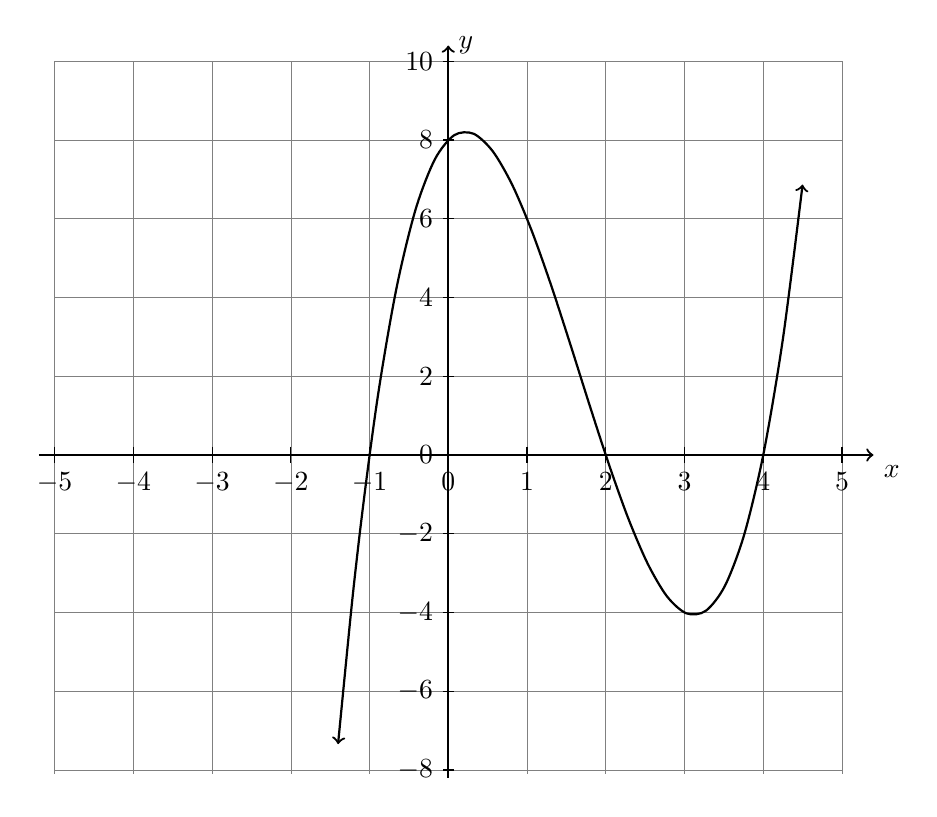
\begin{tikzpicture}[x=1cm, y=0.5cm]
    \draw [help lines] (-5,-8.1) grid (5,10);
    \draw [thick, ->] (-5.2,0) -- (5.4,0) node [below right] {$x$};
    \draw [thick, ->] (0,-8.2)--(0,10.4) node [right] {$y$};
    \foreach \x in {-5,...,5}
        \draw[shift={(\x,0)}] (0,3pt)--(0,-3pt) node[below] {$\x$};
    \foreach \y in {-8,-6,...,10}
        \draw[shift={(0,\y)}] (2pt,0pt)--(-2pt,0pt) node[left]  {$\y$};
    \draw [<->,thick,smooth,domain=-1.4:4.5] plot(\x,{(\x)^3-5*(\x)^2+2*(\x)+8});
\end{tikzpicture}

\begin{enumerate}
  \item Write down the $y$-intercept.
  \item Show that $f(0)$ is the $y$-intercept by substituting $x=0$ into the function $f(x)$.\vspace{1cm}
  \item Write down the $x$-intercepts.
  \item Show that $2$ is an $x$-intercept because $x=2$ is a solution to $f(x)=0$.\vspace{1cm}
  \item What is the end behavior?
  \begin{enumerate}
      \item As $x\xrightarrow{}+\infty$ does $y\xrightarrow{}+\infty \text{ or } -\infty$?
      \item As $x\xrightarrow{}-\infty$ does $y\xrightarrow{}+\infty \text{ or } -\infty$?
  \end{enumerate}
  \item Label the local maximum and local minimum as ordered pairs (approximate the values).
  \item Slope: on the $x$-axis below, label the portion of the domain where $f$ is increasing with pluses (``+") and decreasing with negative signs (``-"). Mark the extema (maximum and minimum) with zeros since $f(x)$ is horizontal at those points.
  \item Write down the intervals the function is increasing and decreasing.
\end{enumerate}
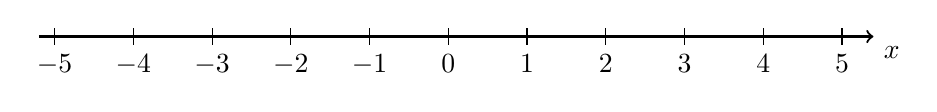
\begin{tikzpicture}[x=1cm]
    \draw [thick, ->] (-5.2,0) -- (5.4,0) node [below right] {$x$};
    \foreach \x in {-5,...,5}
        \draw[shift={(\x,0)}] (0,3pt)--(0,-3pt) node[below] {$\x$};
\end{tikzpicture}

\newpage
\item A rectangular picture frame has a perimeter of 320 centimeters.
    \begin{enumerate}
        \item Let $x$ be the width of the frame in cm. Find an expression in terms of $x$ for the height of the frame. \vspace{2cm}
        \item Find an expression for the area of the frame, $A \,\rm{cm}^2$, in terms of $x$.  \vspace{2cm}
        \item Plot a graph of how the area varies with width. Mark the coordinates of the vertex and $x$-axis intercepts.
        \item Explain what the coordinates of the vertex represent in the context of the situation. \vspace{4cm}
    \end{enumerate}
    \begin{center}
    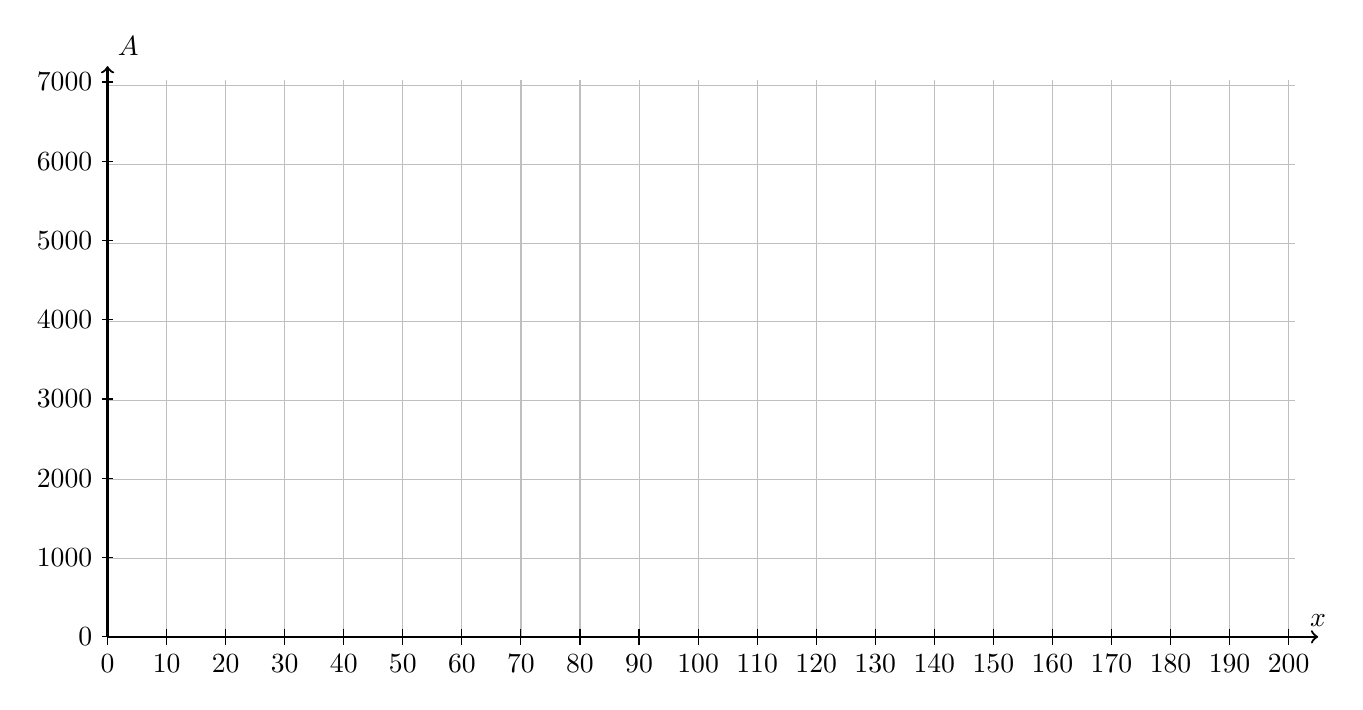
\begin{tikzpicture}[x=0.075cm, y=0.001cm]
        \draw [thin, color=lightgray, xstep=0.75cm,ystep=1.0cm] (0,0) grid (201,7020);
        \foreach \x in {0,10,...,200}
            \draw[shift={(\x,0)}] (0,3pt)--(0,-3pt) node[below]{$\x$};
        \foreach \y in {0,1000,...,7000}
            \draw[shift={(0,\y)}] (2pt,0pt)--(-2pt,0pt) node[left]{$\y$};
        \draw [thick, ->] (0,0) -- (+205,0) node [above] {$x$};
        \draw [thick, ->] (0,0) -- (0,7200) node [above right] {$A$};
        %\draw [thick, <->,smooth,domain=0:160] plot(\x,-\x*\x+160*\x);
    \end{tikzpicture}
    \end{center}
    
\newpage
Sum of an arithmetic series: $\displaystyle S_n=\frac{n}{2}(2u_1+d(n-1))$
\item The first four terms of an arithmetic sequence are 6, 10, 14, 18. 
\begin{enumerate}
    \item Write down the common difference, $d$. \vspace{0.5cm}
    \item Show the the sum to $n$ terms can be written as $2n^2+4n$.\vspace{3cm}
    \item The sum of $n$ terms is 880. Write a quadratic equation to represent this information. Rearrange to equal zero and plot the function, showing the $x$-intercepts and the coordinates of the vertex.\vspace{2cm}
    \item State what information the positive $x$-intercept tells you about the sequence.
\end{enumerate}
\vspace{3cm}
\begin{center}
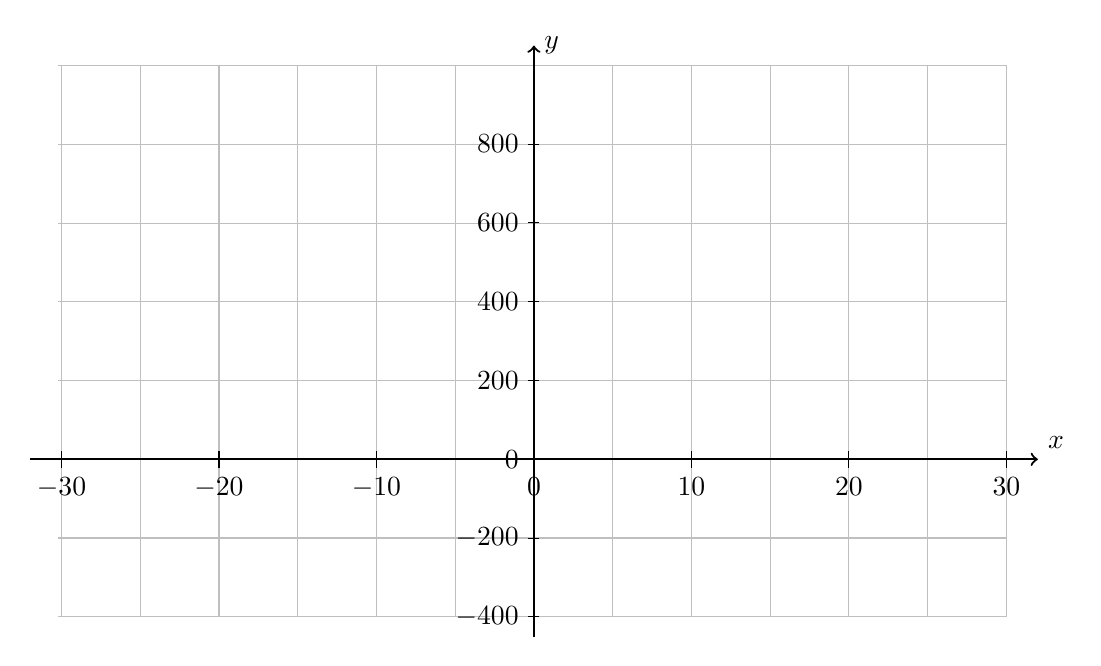
\begin{tikzpicture}[x=0.2cm, y=0.005cm]
    \draw [thin, color=lightgray, xstep=1.0cm,ystep=1.0cm] (-30.2,-400) grid (30,1000);
    \foreach \x in {-30,-20,...,30}
        \draw[shift={(\x,0)}] (0,3pt)--(0,-3pt) node[below] {$\x$};
    \foreach \y in {-400,-200,...,800}
        \draw[shift={(0,\y)}] (2pt,0pt)--(-2pt,0pt) node[left]  {$\y$};
    \draw [thick, ->] (-32,0) -- (+32,0) node [above right] {$x$};
    \draw [thick, ->] (0,-450) -- (0,1050) node [right] {$y$};
    %\draw [thick, <->,smooth,domain=-25:22] plot(\x,2*\x*\x+4*\x-880);
\end{tikzpicture}
\end{center}

\end{enumerate}
\end{document}



\item The function $g(x)=-x^3-7x^2-14x-8$ is shown on the graph.
      %$g(x)=(x-2)(x-4)(x+1)$

\begin{tikzpicture}[scale=.75]
  \tkzInit[xmin=-5,xmax=5,ymin=-10,ymax=10,ystep=2]
  \tkzGrid
  \tkzAxeXY
  %\tkzFct[color=blue,thick,domain = -5:5]{-x**3-7*x**2-14*x-8};
  \draw [<->,thick,smooth,domain=-4.7:0.12] plot(\x,{0.5*(-(\x)^3-7*(\x)^2-14*(\x)-8)});
\end{tikzpicture}

\begin{enumerate}
    \item Write down the $y$-intercept.
    \item Show that $f(0)$ is the $y$-intercept by substituting $x=0$ into the function $f(x)$.\\*[20pt]
    \item Write down the $x$-intercepts.
    \item Show that $-1$ is an $x$-intercept because $x=-1$ is a solution to $f(x)=0$.\\*[20pt]
    \item What is the sign of the leading coefficient?\\* What is the end behavior?
    \begin{enumerate}
        \item As $x\xrightarrow{}+\infty$ does $y\xrightarrow{}+\infty \text{ or } -\infty$?
        \item As $x\xrightarrow{}-\infty$ does $y\xrightarrow{}+\infty \text{ or } -\infty$?
    \end{enumerate}
    \item Label the local maximum and local minimum as ordered pairs (approximate the values).
    \item Slope: on the $x$-axis below, label the domain as increasing, decreasing, or horizontal (with ``+", ``-", \& ``0"), and state the respective intervals. \\*[10pt]
\end{enumerate}

\begin{tikzpicture}[scale=.75]
  \tkzInit[xmin=-5,xmax=5]
  \tkzAxeX
\end{tikzpicture}

\newpage
\item Given the function $h(x)=x^3+2x^2-5x-6$.

\begin{enumerate}
    \item Write down the $y$-intercept. Mark it on the plot.
    \item Show that $-1$ is an $x$-intercept because $x=-1$ is a solution to $f(x)=0$. Mark $(-1, 0)$ on the graph as an $x$-intercept.\\*[20pt]
    \item The other $x$-intercepts are $-3$ and $+2$. Mark them on the plot.

    \begin{tikzpicture}[scale=1.0]
      \tkzInit[xmin=-5,xmax=5,ymin=-10,ymax=10,ystep=2]
      \tkzGrid
      \tkzAxeXY
      %\tkzFct[color=blue,thick,domain = -5:5]{x**3+2*x**2-5*x-6};
    \end{tikzpicture}

    \item What is the sign of the leading coefficient, positive or negative? Hence, what is the function's end behavior?
    \begin{enumerate}
        \item As $x\xrightarrow{}+\infty$ does $y\xrightarrow{}+\infty \text{ or } -\infty$?
        \item As $x\xrightarrow{}-\infty$ does $y\xrightarrow{}\infty \text{ or } -\infty$?
    \end{enumerate}
    \item Using the intercepts and end behavior, sketch the curve.
    \item Graph the function on a calculator. Is the shape of your sketch approximately correct?
\end{enumerate}

